\documentclass[10pt]{article}
 \usepackage[usenames]{color} %used for font color
\usepackage{amssymb} %maths
\usepackage{amsmath} %maths
\usepackage{mathtools} % MATHS.
\usepackage{blkarray}
\usepackage[margin=0.2in]{geometry}
%\usepackage{breqn}
\usepackage[utf8]{inputenc} %useful to type directly diacritic
%characters
\usepackage{pdflscape}
\usepackage{subfig}

\usepackage{breakcites}
\usepackage{microtype}




\begin{document}
    \begin{figure}
      \centering
      \subfloat[][$e=1$]{\noindent
        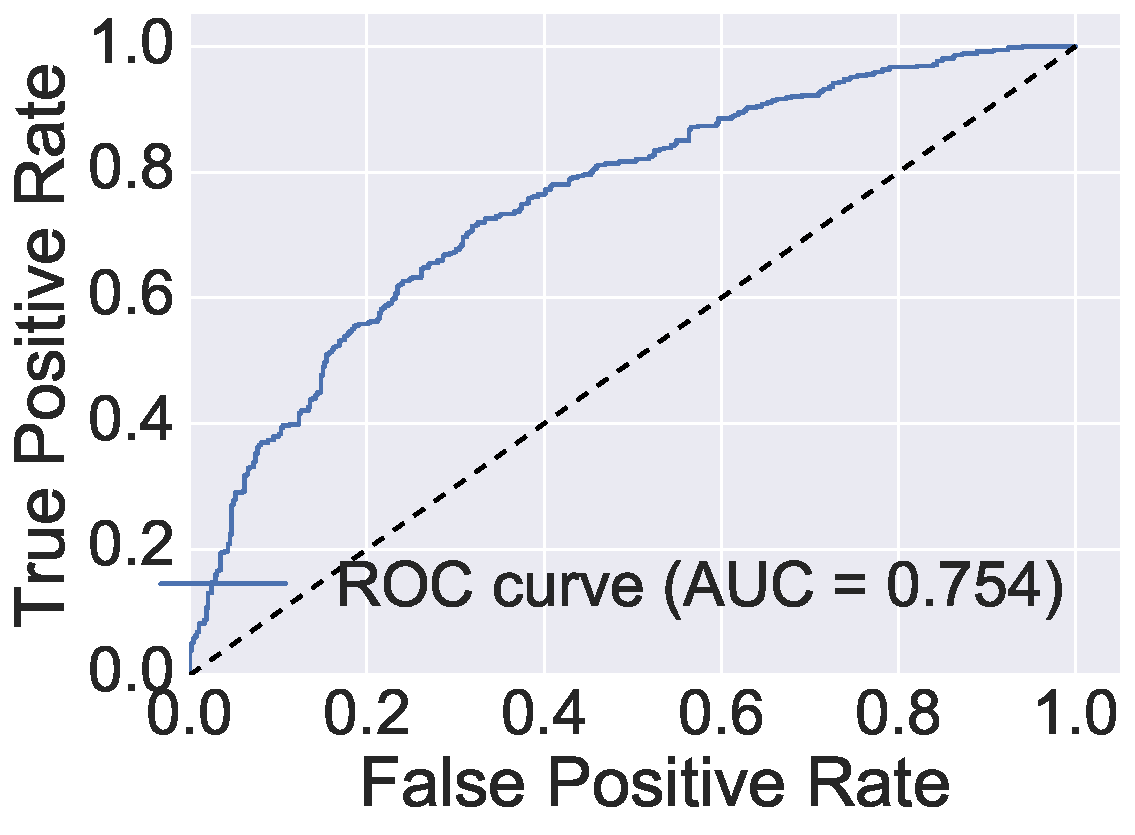
\includegraphics[width=.4\textwidth]{/Users/ijoseph/Documents/Work/Graduate-Thesis/TeX/figures/ch4/mfaa__roc__w_2_psi_2.pdf}}% 
      \qquad \\
      \subfloat[][$e=1.25$]{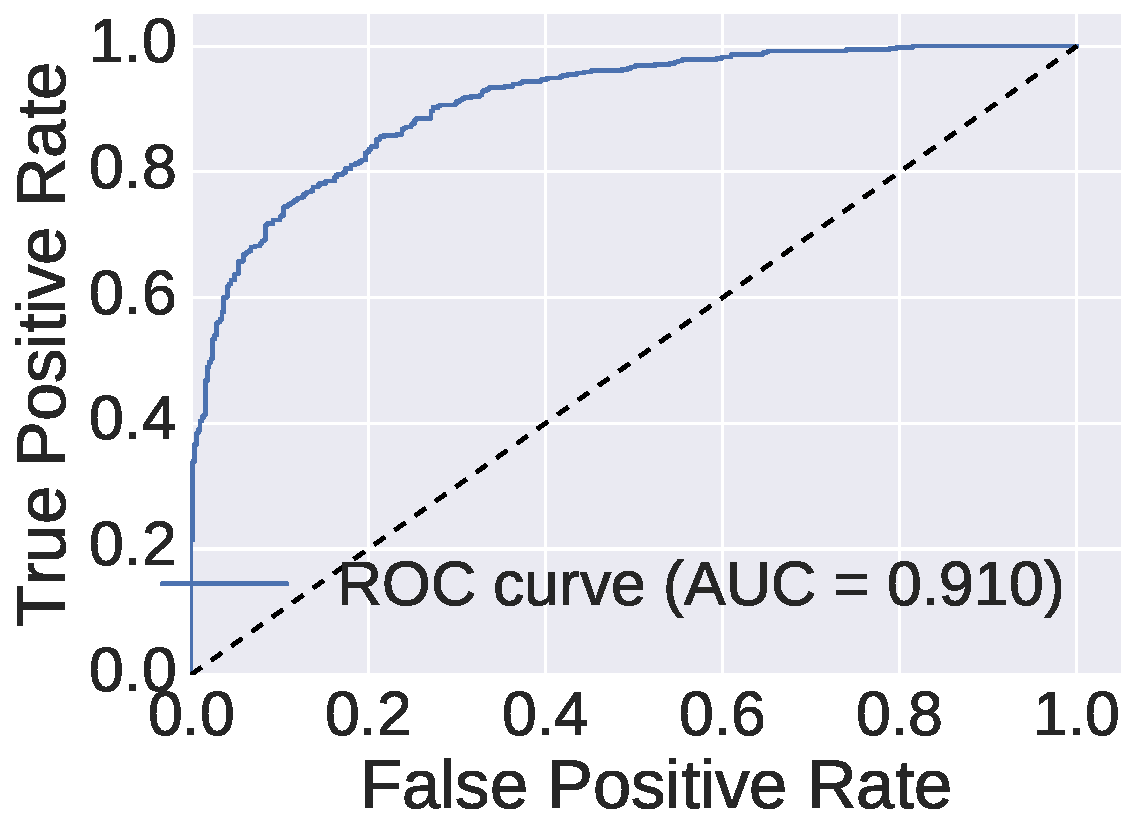
\includegraphics[width=.4\textwidth]{{/Users/ijoseph/Documents/Work/Graduate-Thesis/TeX/figures/ch4/mfaa__roc__w_3_psi_2}.pdf}}
      \qquad \\
      \subfloat[][$e=10$]{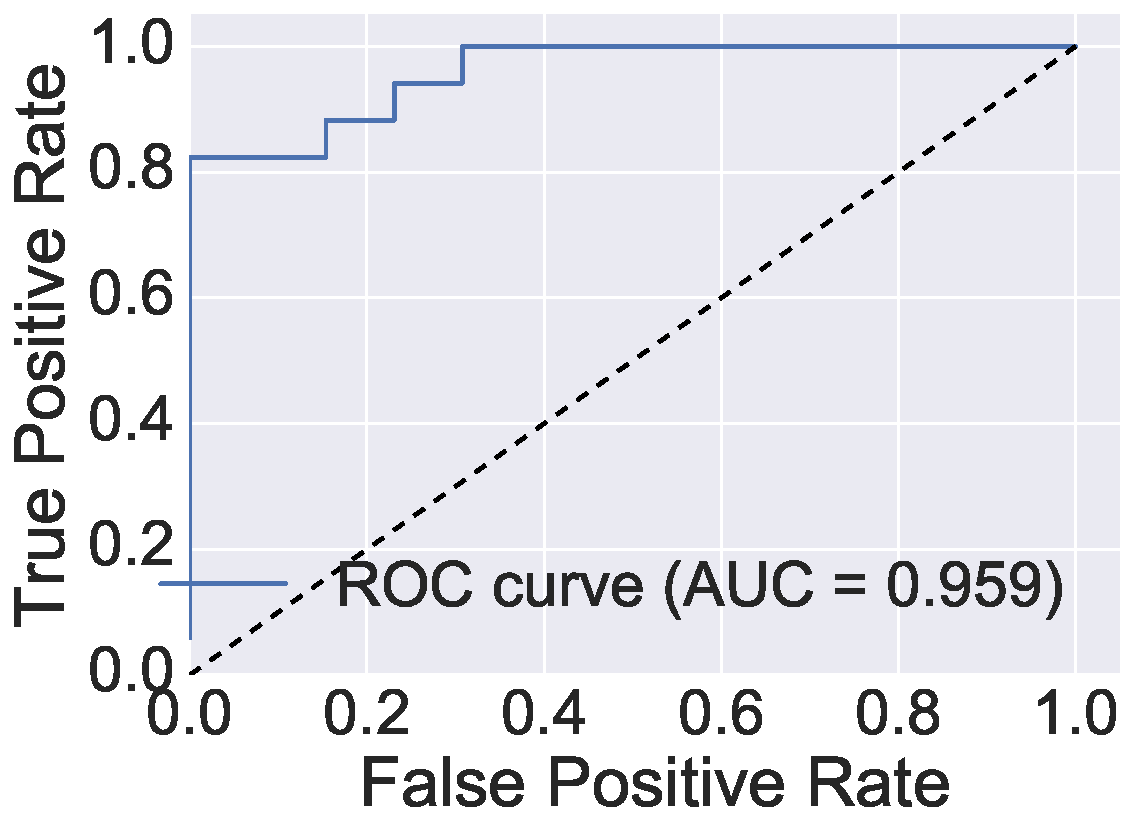
\includegraphics[width=.4\textwidth]{{/Users/ijoseph/Documents/Work/Graduate-Thesis/TeX/figures/ch4/mfaa__roc__w_20_psi_2}.pdf}}
      \caption{HFAM ROC curves from HFAM-simulated $N=30, p=10$}
    \end{figure}

    \begin{figure}
      \centering
      \subfloat[][$e=1$]{\noindent
        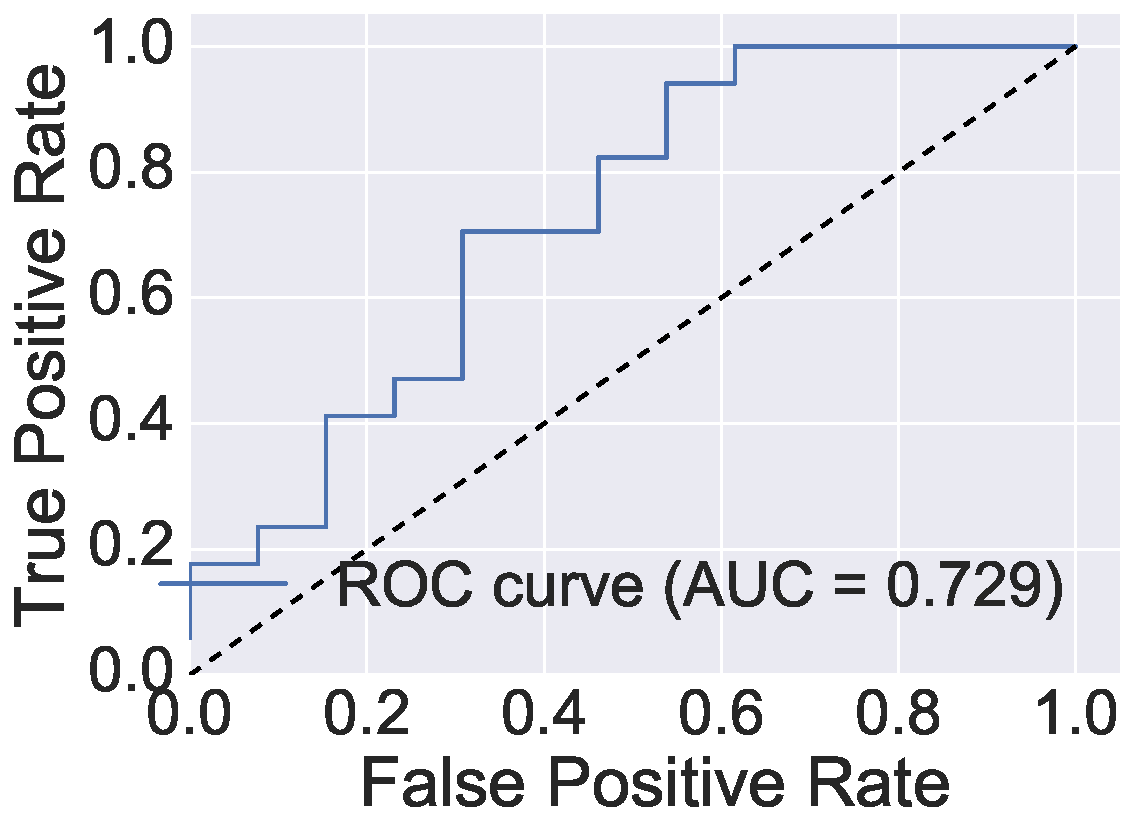
\includegraphics[width=.4\textwidth]{/Users/ijoseph/Documents/Work/Graduate-Thesis/TeX/figures/ch4/log_reg__roc__w_2_psi_2.pdf}}% 
      \qquad \\
      \subfloat[][$e=1.25$]{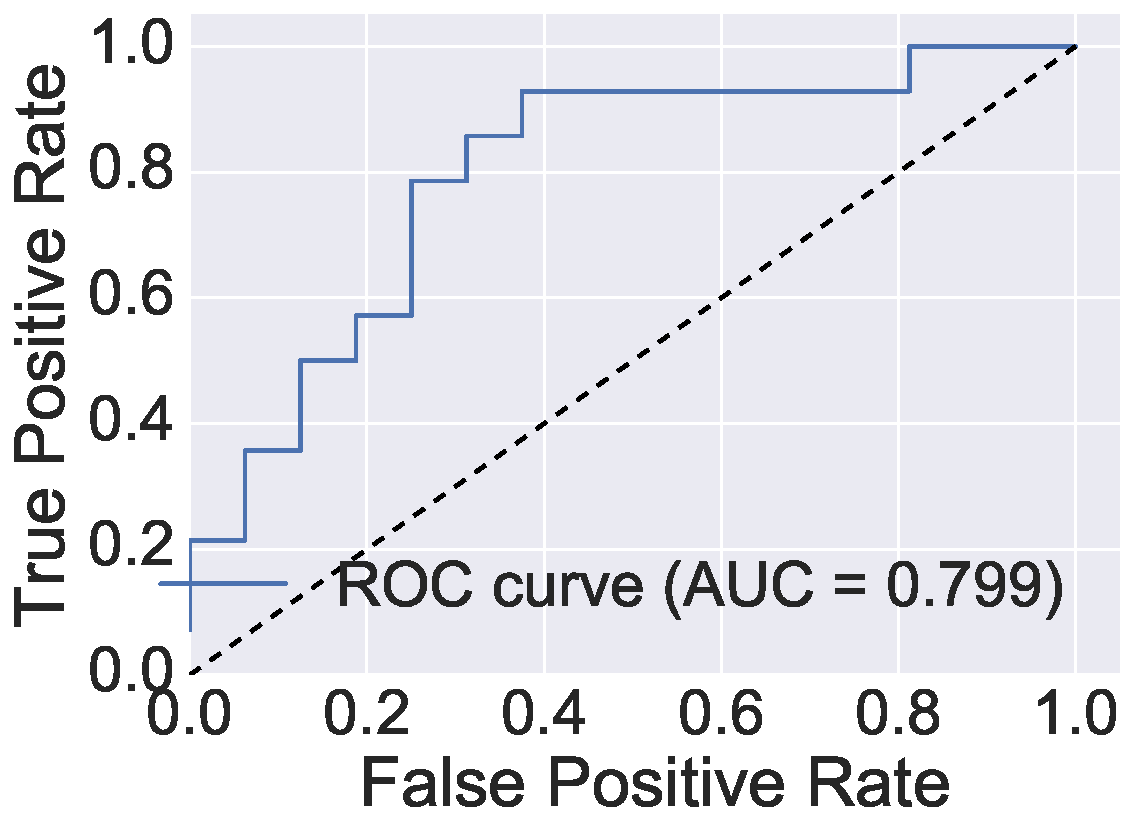
\includegraphics[width=.4\textwidth]{{/Users/ijoseph/Documents/Work/Graduate-Thesis/TeX/figures/ch4/log_reg__roc__w_3_psi_2}.pdf}}
      \qquad \\
      \subfloat[][$e=10$]{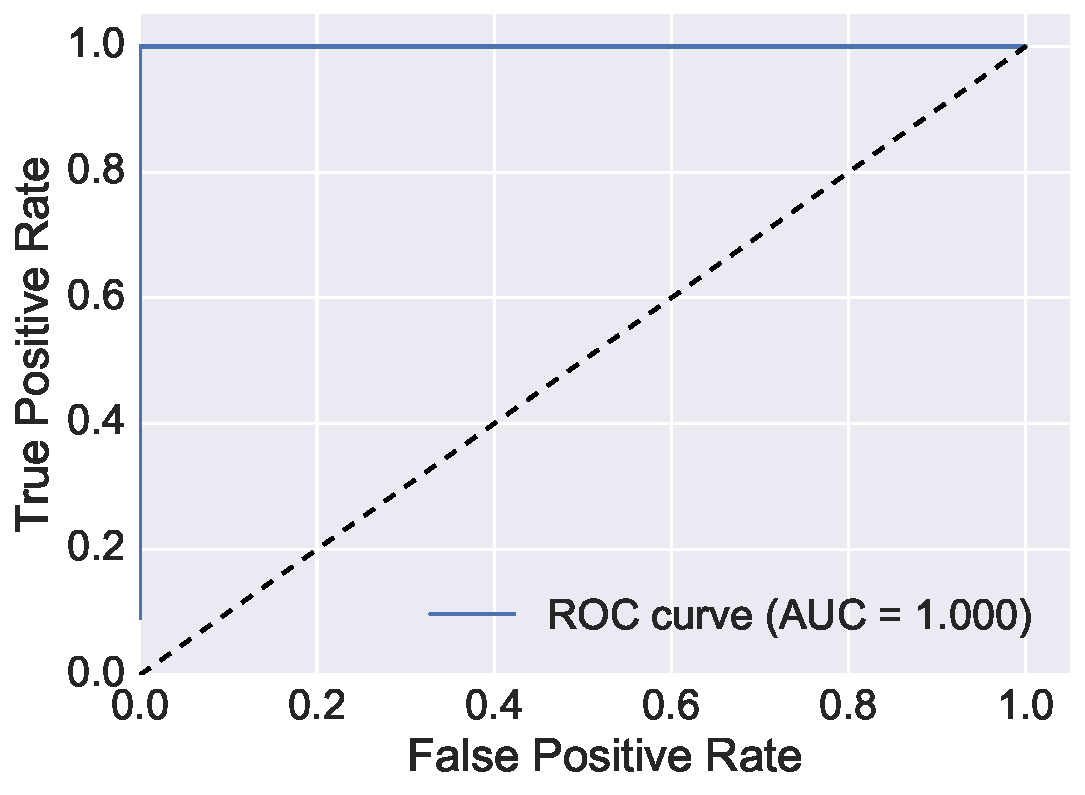
\includegraphics[width=.4\textwidth]{{/Users/ijoseph/Documents/Work/Graduate-Thesis/TeX/figures/ch4/log_reg__roc__w_20_psi_2}.pdf}}
      \caption{Logistic regression ROC curves from HFAM-simulated $N=30, p=10$}
    \end{figure}    


    \begin{figure}
      \centering
      \subfloat[][$e=1$]{\noindent
        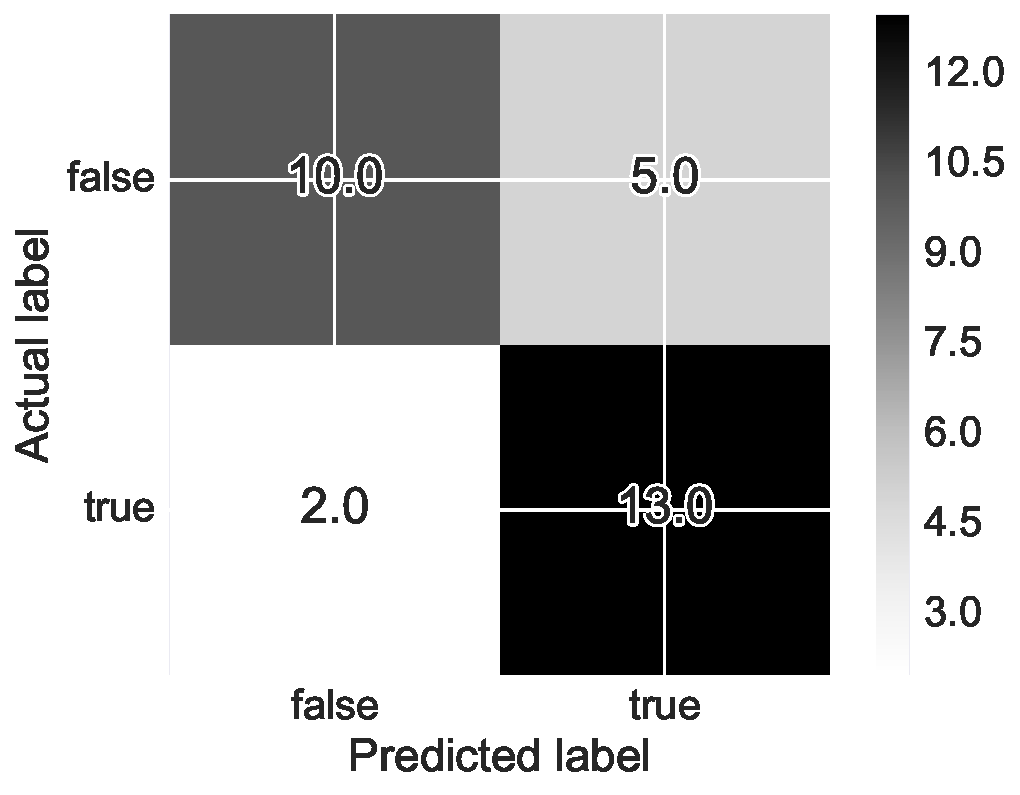
\includegraphics[width=.4\textwidth]{/Users/ijoseph/Documents/Work/Graduate-Thesis/TeX/figures/ch4/mfaa__confusion__w_2_psi_2.pdf}}% 
      \qquad \\
      \subfloat[][$e=1.25$]{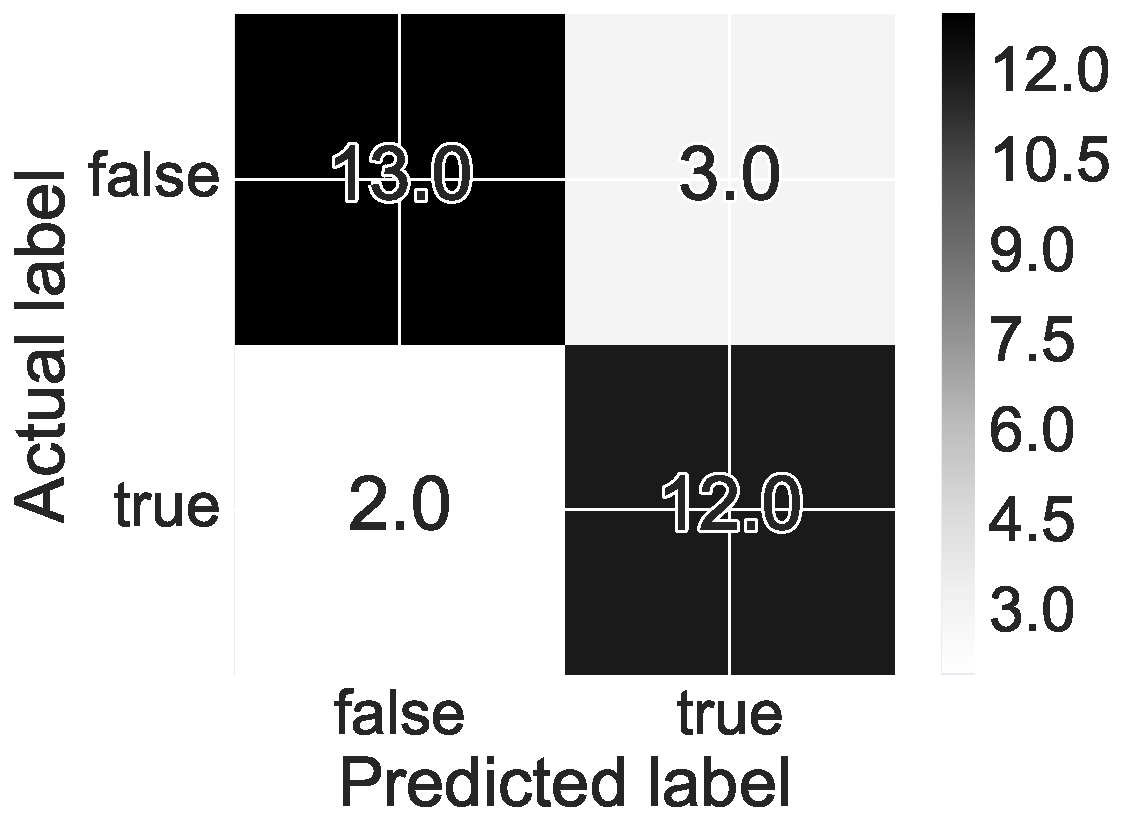
\includegraphics[width=.4\textwidth]{{/Users/ijoseph/Documents/Work/Graduate-Thesis/TeX/figures/ch4/mfaa__confusion__w_3_psi_2}.pdf}}
      \qquad \\
      \subfloat[][$e=10$]{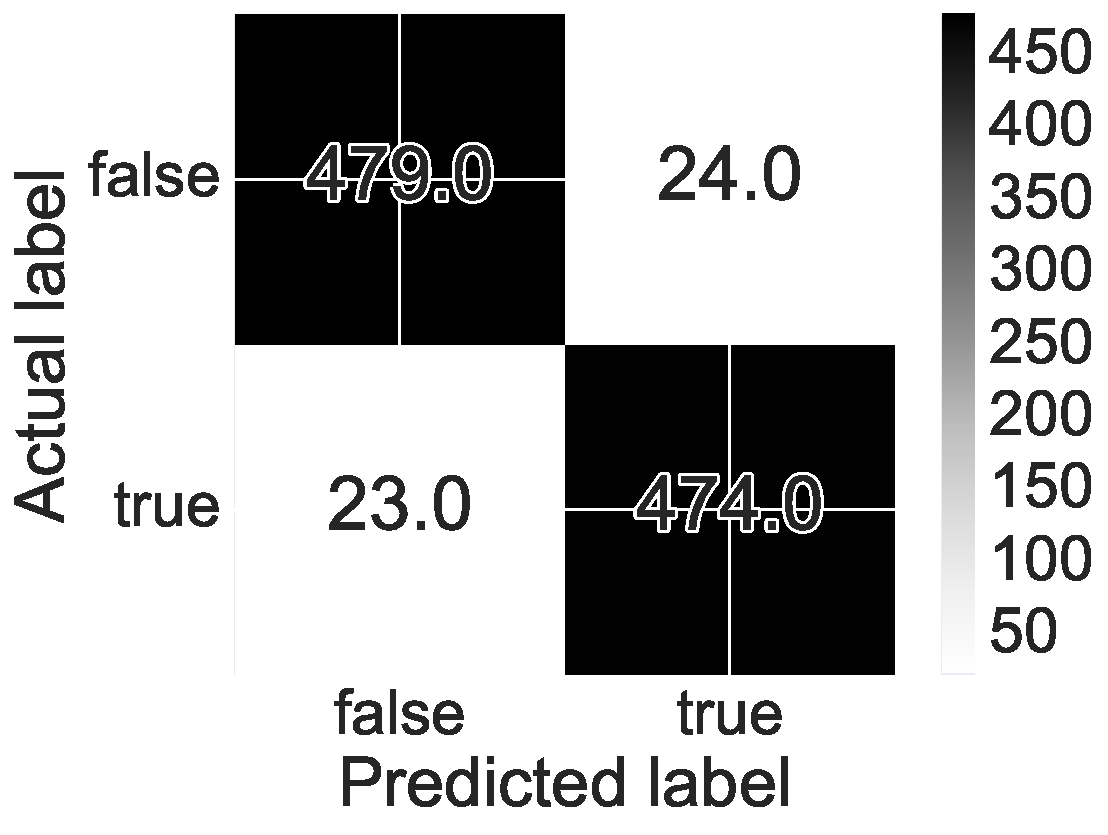
\includegraphics[width=.4\textwidth]{{/Users/ijoseph/Documents/Work/Graduate-Thesis/TeX/figures/ch4/mfaa__confusion__w_20_psi_2}.pdf}}
      \caption{HFAM confusion matrices from HFAM-simulated $N=30, p=10$}
    \end{figure}


    \begin{figure}
      \centering
      \subfloat[][$e=1$]{\noindent
        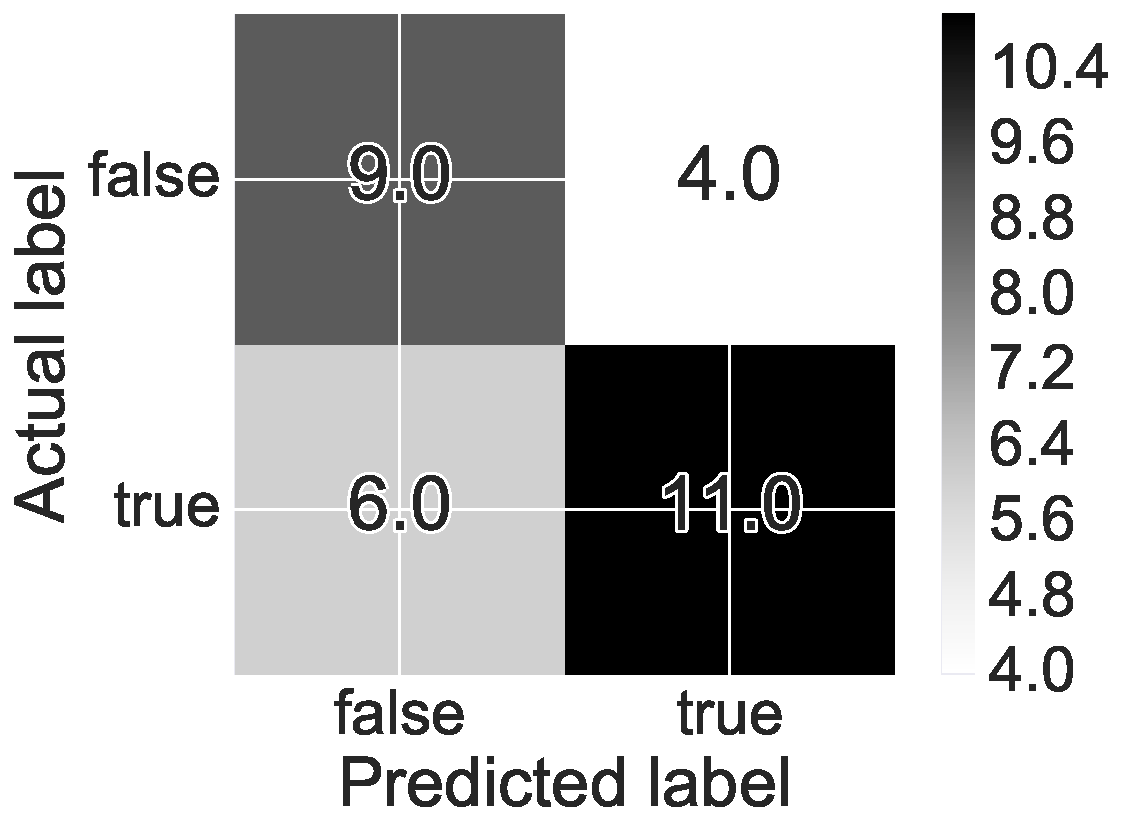
\includegraphics[width=.4\textwidth]{/Users/ijoseph/Documents/Work/Graduate-Thesis/TeX/figures/ch4/log_reg__confusion__w_2_psi_2.pdf}}% 
      \qquad \\
      \subfloat[][$e=1.25$]{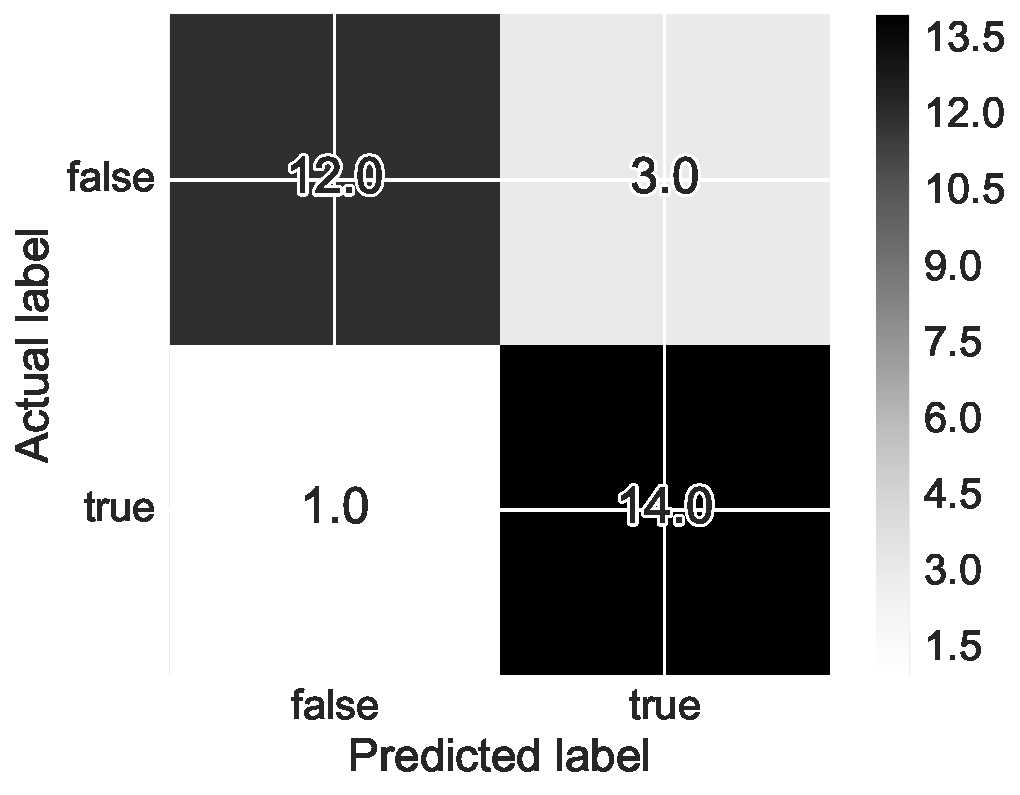
\includegraphics[width=.4\textwidth]{{/Users/ijoseph/Documents/Work/Graduate-Thesis/TeX/figures/ch4/log_reg__confusion__w_3_psi_2}.pdf}}
      \qquad \\
      \subfloat[][$e=10$]{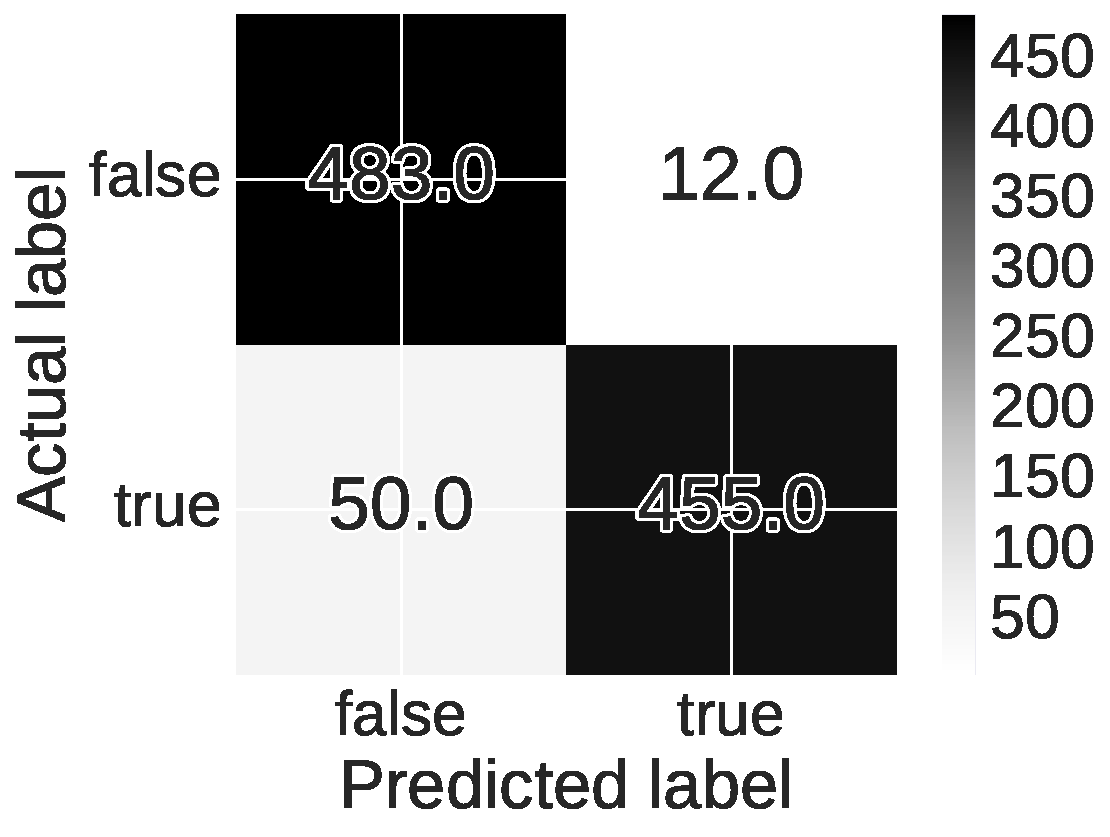
\includegraphics[width=.4\textwidth]{{/Users/ijoseph/Documents/Work/Graduate-Thesis/TeX/figures/ch4/log_reg__confusion__w_20_psi_2}.pdf}}
      \caption{Logistic regression confusion matrices from HFAM-simulated $N=30, p=10$}
    \end{figure}
    

    
    


    





\end{document}